% ------------------------------------------------------------------------ %
% !TEX encoding = UTF-8 Unicode
% !TEX TS-program = pdflatex
% !TEX root = ../Tesi.tex
% !TeX spellcheck = en_US
% ------------------------------------------------------------------------ %
%
% ------------------------------------------------------------------------ %
% 	PROPOSED SOLUTION
% ------------------------------------------------------------------------ %
%
\chapter{Proposed Solution}
%
\label{cap:proposedsolution}
%
% ------------------------------------------------------------------------ %
%
\par In this chapter the development of the solution will be reported step by step, with a full use case. The chapter starts with a list of similar solutions already developed, highlighting the differences between them and my thesis work. The remaining part is composed of tree mains sections: the first explains the choice of the network, the architecture, the naming service, etc. It lays the foundations for the second part: the definition of the Liquid Android middleware, or better the structure of what will do the magic: intercept, encapsulate, spread, and generate distributed intents in the network so made. The two parts are closely related, therefore their relation was taken into account when I made my choice.\\
The real implementation of the valid solution is left for the next chapter.
%

\section{Existing Solutions }
Android distributed systems already exists as specific purposes application to be installed on multiple devices, what it is different to the aim of this thesis work is that these application are closed source projects that can not be reused to build other purposes systems and there is not a coherent framework, library or API to be used to easily build such systems.
I want to give some examples pointing out the nice features have this native distributed Android systems.
\subsection{Boincoid and HTC Power to Give}
Boincoid and HTC Power to Give are Android application which aim is  to exploit Android devices computation power to contribute to scientific discoveries by doing some task. The common idea is to have an Android distributed supercomputer which can handle heavy task and compute tons of data for larger purposes.\\
BOINC is an open-source software platform for computing using volunteered resources \cite{boinc2017open}. It is a program that lets you donate your idle computer time to science projects. Boincoid is a port of the BOINC platform to the Android operating system. The result is an Android BOINC client that behaves exactly like the original one.\\
HTC Power to give is very similar to Boincoid, it is a \textit{CSR (Corporate Social Responsibility)} initiative from HTC that has been jointly developed with Dr. David Anderson at University of California, Berkeley. Using the HTC Power To Give, owners of Android OS smartphones can choose to ‘give back’ by supporting key research projects around the world. Scientific research often requires a vast amount of processing power for data modeling and analysis. HTC Power To Give, supported by the world’s largest single distributed volunteer computing platform BOINC, lets users donate their unused smartphone computing power to science programmes across diverse fields as astronomy, environment, medicine and physics \cite{htc2017power}.
 
\subsection{Plex for Android}
Plex platform is a great, maybe the best, media content streaming distributed system platform. It is mainly composed of two components, the media server, and a client with which enjoy the contents.
\begin{figure}[h]
	\centering
	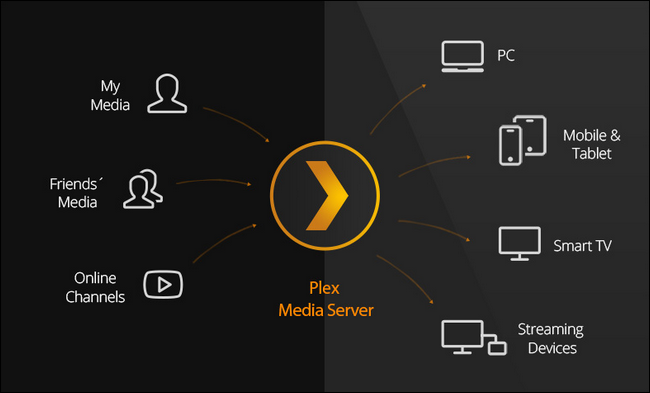
\includegraphics[width=.8\textwidth]{plex}
	\caption{Plex Platform}
	\label{fig:4.1}
\end{figure}
The Plex Media Server either running on Windows, macOS, Linux, FreeBSD or a NAS which organizes audio (music) and visual (photos and videos) content from personal media libraries and streams it to their player counterparts.
The players can either be the Plex Apps available for mobile devices, smart TVs, and streaming boxes, or the web UI of the Plex Media Server called Plex Web App, or the old Plex player called Plex Home Theater.\\
In particular Plex for Android application can connect to the media server to play its content and in addition it can search for Plex players in a LAN and send streamed content such as videos, movies or photo, to another player that can be also an Android device. In this way the Android Plex application client can behave like the Liquid Android system i want to develop. It can send a sort of \textit{Android intent}, to reproduce a media, from one device to another, and then it can send commands such as pause, rewind, forward and so on. The limits of such a system are that it is possible to send, and play, only multimedia contents, and only to devices which have the Plex app activity in foreground on the device.

\subsection{Goolgle Home and Cast API}
Google itself provides an application to control and send contents form an Android device, to some special devices in home network. \textit{Google Home} is an Android application which can find, setup, manage and control, Google's home devices like the \textit{Google Chromecast}. In this way is easy to setup and control and Android distributed system in which user can sent multimedia contents and command to the Google Home devices in the LAN. For these reason Google provides a development library, included in the Android framework, called \textit{Cast API} with which it is easy, for a developer, to build applications that can send multimedia streams to other Google devices specifically built for these purposes.\\
Also in this case the limitation is the kind of content, only multimedia, and also the type of devices involved which are limited number of special purposes devices.

\subsection{DroidMote and Remote control systems }
If we consider the possibility to control remote devices in a LAN, there are actually many different kind of applications that can do that also in an Android environment.
DroidMote is probably the most complete application to control remotely an Android device from another one. It is composed by two parts, the server, to be installed in the device to be controlled, and the client, to be installed in the one which controls. With this application is possible to control entirely the device running the server component: is it possible to open applications, perform tasks, open system settings and so on.\\
These kind of systems are capable to generate local intents in remote devices over a LAN but in a completely different way from I want to develop the solution to the given problem. In this case the \textit{controller} is explicitly controlling the remote device as it is using only the \textit{controlled} one. These systems are solution only to the problem of remote control, they can not exploit distributed Android devices computation power, in fact in an environment like this Android devices are not cooperating to perform task but one of them is only controlling another one.
\section{General Idea}
\par To better explain what I consider solution for my work it is important to
understand the playground to my work. As said in the previous chapter, \ref{cap:probanalysis}, I
am trying to extend the Android operating system by adding some functionalities to make it similar to a distributed OS, without the need of rooting it or change its standard working mechanism and components, staying in the 7th layer of the ISO/OSI stack , the application layer. Using already developed and operating tools, and respecting all the above listed constraints I am going to make mobile devices in a LAN network communicate and cooperate like they were using a single coherent distributed operating system.
In order to understand what is needed and how it is possible to solve the problem
it is fundamental to understand the type of stack and the network structure
we have to face, and standard Android working principle, in particular the intent resolution mechanism already described in \figurename~\ref{fig:2.4}.\\
Only having clear in mind the problem and its structure it is possible to find the best possible solution. In particular it is possible to decompose the main problem in some sub-problems, which can be understood as general steps in doing similar works of extending a mobile OS to become a distributed OS:
\begin{itemize}
	\item Network architecture, that is the structure and the classification of the nodes involved in the distributed system. As previously said it has to be as reliable  as possible and allow dynamic connection due to the fact that nodes are mobile devices and can be easily moved in and out the network range.
	\item Communication model, that is the way in which involved actors perform the communication. It has to be compliant to M2M, and possibly to H2M communication, and as lightweight as possible to allow fast exchange of messages and data between the network nodes.
	\item Data model, as discussed before in the chapter \ref{cap:statoarte}, when building distributed systems it is also important to guarantee that data are managed correctly by adopting a consistency policy.
\end{itemize}
It is also necessary to identity the main actor involved in the problem, they are mainly two:
\begin{itemize}
	\item Server application, it is the main actor of this thesis work, it must be an Android application which once installed on a compatible Android device can receive resolve and forward Android intents. It contains the logic and the controllers needed to handle the network structure, find other devices in the network, send and receive messages. It is responsible of resolving all the three sub-problems described above. The server application has also the double function of receiving a message from the network and translate it in a local intent to be resolved by the Android operating system, but also it can act as a client by forwarding a received intent from a third party client application to another server in the net, by encapsulating the intent in a network message.
	\item Clients, can be applications developed in several ways, they are those which are asking to the so called servers to complete task for them. In this case clients could be any kind of third party Android application installed in the device, also running the server component, generating implicit Android intents that need to be resolved by the OS. 
\end{itemize}
Once defined the main actors of the problem I am facing, the next step is to understand how they can interact and communicate. As previously described defining the problematic scenarios in the chapter \ref{cap:probanalysis}, the Liquid Android middleware in the best case would be a system service which users can control to distribute intents in the local network by using the WiFi chip of the devices.
 \begin{figure}[h]
	\centering
	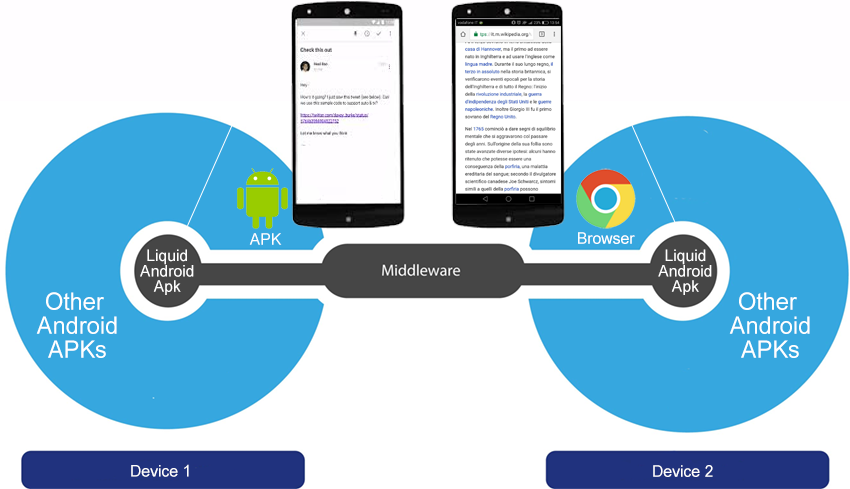
\includegraphics[width=.9\textwidth]{esempio1}
	\caption{Liquid Android working example}
	\label{fig:4.2}
\end{figure}
The \figurename~\ref{fig:4.2} shows exactly how the middleware is supposed to work. In the figure the two devices are both supposed to be connected to the same local network \textit{(they are under the same WiFi access point)} and they are executing any standard Android OS version starting from 4.4 KitKat \textit{(API level 19)}. The so called, in the picture, \textit{Device 1} is executing a third party application activity \textit{(a client)}  which contains a valid clickable URL link. By clicking a link, typically, Android applications generate an implicit intent asking to the OS to open and show the page linked by the URL. Usually, in the absence of other applications capable of solving this kind of implicit intent, the process ends with the opening of a browser in the same device, which opens the URL in one of its activities. In this case the Liquid Android application server, installed on both devices, should to tell the OS that it can handle that implicit intent, find the other devices in the net, in this case the so called \textit{Device 2}, le the user choose with which device complete the task, convert the intent in a network message and send it to that device. Once the message arrived to the \textit{Device 2} the Liquid Android middleware server application is responsible to translate again the received message into the starting implicit intent sent by the \textit{Device 1} and to start the very same resolution mechanism for that intent by its own Android operating system, which should end by the opening of a browser activity to view the page.\\
It is clear that a solution for this scenario would be also, once implemented, a solution for the second problematic scenario proposed in \ref{devAPI}. In fact we can consider the development of an API to build native Android distributed systems as a sub problem of the first one, already described above and in \ref{middlewarescenario}. The implemented version of the general solution could be also used as a library to implement special purposes similar systems by simply extending my framework and including its implemented Java classes in other Android applications projects. For these reasons in developing the solution I will try to make it as clear as possible, and to parametrize as far as possible the settings variable of my framework to make it easily extensible and ready to use buy other Android developers.\\
I would like now to list the goals that my work has to match, in order to be a valid proposal for solving the given problem. These goals are not to be intended as set in stone, they are the general motivation that leads to construct a prototype of the proposed software architecture. According to my thoughts during the development, it is possible to identify the following goals:
\begin{itemize}
	\item The middleware must work without any proprietary application: it has to interface itself to the upper layer without installing any other application of any vendor in the owned device. It must be completely neutral to the market, it must work with any version of the Android operating system starting from the API level 19, also with Android customized versions developed by device maker like Samsung, LG, Huawei and any other brand. It is the fundamental requirement to create heterogeneous applications and to separate the various closed solutions of today and an open solution for everyone in the future.
	\item The middleware has to simplify the life of the developer, he should not have to worry too much about the substrates, he should be able to fast prototype. The developer should see my framework as help for his work. The idea is to provide a ready to use service, with which it is possible create new application by exploiting it.
	\item The middleware should offer the user the possibility to access directly to other devices in the network without the need of configure anything. Users, once installed the middleware should use its functionalities of receiving/forwarding intents in a transparent way, in the same way they use other applications and with the same mechanism they learned by using the standard Android operating system.
\end{itemize}
The next sections contain all the steps necessary to have a full working system.
Firstly I would solve the, let me call it \textit{general theoretical problem} by dividing it as discussed above and providing the solution for each of them, taking into account also the data management scenario. Then I would like present the structure of the development API, while the actual implementation of the working Liquid Android application is left for the next chapter with some working test and a deep analysis.



\section{Liquid Android Framework}



%
% -----------------------------END--------------------------------- %